\documentclass{article}
\usepackage[utf8]{inputenc}
\usepackage{caption}  
\usepackage{geometry}
\usepackage{graphicx}
\usepackage{hyperref}
\usepackage{amsmath}
\usepackage{amssymb}
\usepackage{listings}

\geometry{left=3.0cm,right=3.0cm,top=2.0cm,bottom=2.0cm} 
\captionsetup{margin=10pt,font=small,labelfont=bf,labelsep=endash}

\title{Ugeopgave1}
\author{hjg708}
\date{September 2021}

\begin{document}

\begin{titlepage}
\title{PoP Ugeopgave 2}
\author{Hold 01 \\\\ Aditya Fadhillah \\\\ hjg708}
\date{\today}
\maketitle
\thispagestyle{empty}   
\end{titlepage}


\pagenumbering{arabic} 

\section*{2i0}
\subsection*{Describe the 3 ways an F\# program can be run from the command line (terminal), and discuss the advantages and disadvantages of each method.}
fsharpi \\
fsharpi er en interaktiv tilstand for F\# som giver en resultat med det samme, når brugeren taste noget ind på terminalen efter de har tastet fsharpi. Det vil sige at man ikke behøver noget tekst fil for at køre en kode på fsharpi. fsharpi er virkelig god hvis man bare lige vil lave noget små eksperimenter eller noget hurtigt udregning. Men som regle er fsharpi ikke egnet til lange koder, da den ikke gemmer ens koder, så man skal taste de hele igen for at køre koden en gang til.\\
\\
fsharpi [file name].fsx \\
Her er der så tale om den anden funktion for fsharpi, her compile og udføre fsharpi ens script, så på den måde slipper man for at skulle compile det selv. I den her interaktiv tilstand skal scripten compiles for hver gang programmet udføres, det vil derfor tage væsentlig længere tid hvis man gerne vil køre en script på fsharpi end på fsharpc, når man allerede har compilet filen en gang. Det vil være en fordel at bruge fsharpi hvis man hele tiden laver om på ens script, da man alligevel skal compile en opdateret version af scripten før man kan udføre den. \\
\\
fsharpc [file name].fsx 
\\
mono [file name].exe 
\\
Med denne metode skal man selv compile scripten før man kan udføre den som en .exe fil gennem mono. Første gang man compile og udføre filen, vil det tage længere tid end på fsharpi, men man behøver kun at compile filen en gang i modsætning til fsharpi, som skal compile scripten hver gang. Det vil være en fordel at bruge fsharpc hvis man kun skal compile ens script en gang. \\

\section*{2i1}
\subsection*{Using slicing, write an expression in F\# which extracts the first and the second word from the string hello world. Enter the expression in an .fsx file and compile and run it. Does the program produce output? Explain why or why not.}
(Se filen 2i1.fsx på src/ mappen)
\\
Programmets output er som følge:
\begin{verbatim}
"hello"
"world"
\end{verbatim}
Outputen er lige hvad jeg har forventet da jeg skrev scripten, Jeg definerede først en string som indeholder sætningen "hello world". Og i det med at en string opfører sig som en array kunne jeg isolerer dele af stringen. For at tage det først ord i stringen har jeg brugt, string1.[..4] som betyder at jeg tog fra det første bogstav til det femte (F\# bruger 0-indeksering). For det andet ord har jeg brugt, string1.[6..] som betyder at der tages fra det 7. bogstav til det sidste. De to ord ligger oven på hinanden fordi der blev brugt printfn som laver en ny linje.


\newpage
\section*{2i2} 
\subsection*{Use pen and paper to complete the following table}

\begin{figure}[h!]
\begin{center}
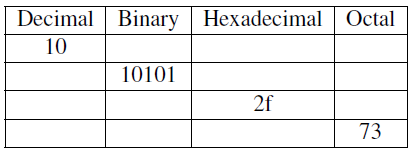
\includegraphics[width=5cm]{2i2.png}
\end{center}
\end{figure}

\subsection*{such that every row represents the same value written on 4 different forms. Include a demonstration of how you converted binary to decimal, decimal to binary, binary to hexadecimal, hexadecimal to binary, binary to octal, and octal to binary.}

\begin{figure}[h!]
\begin{center}
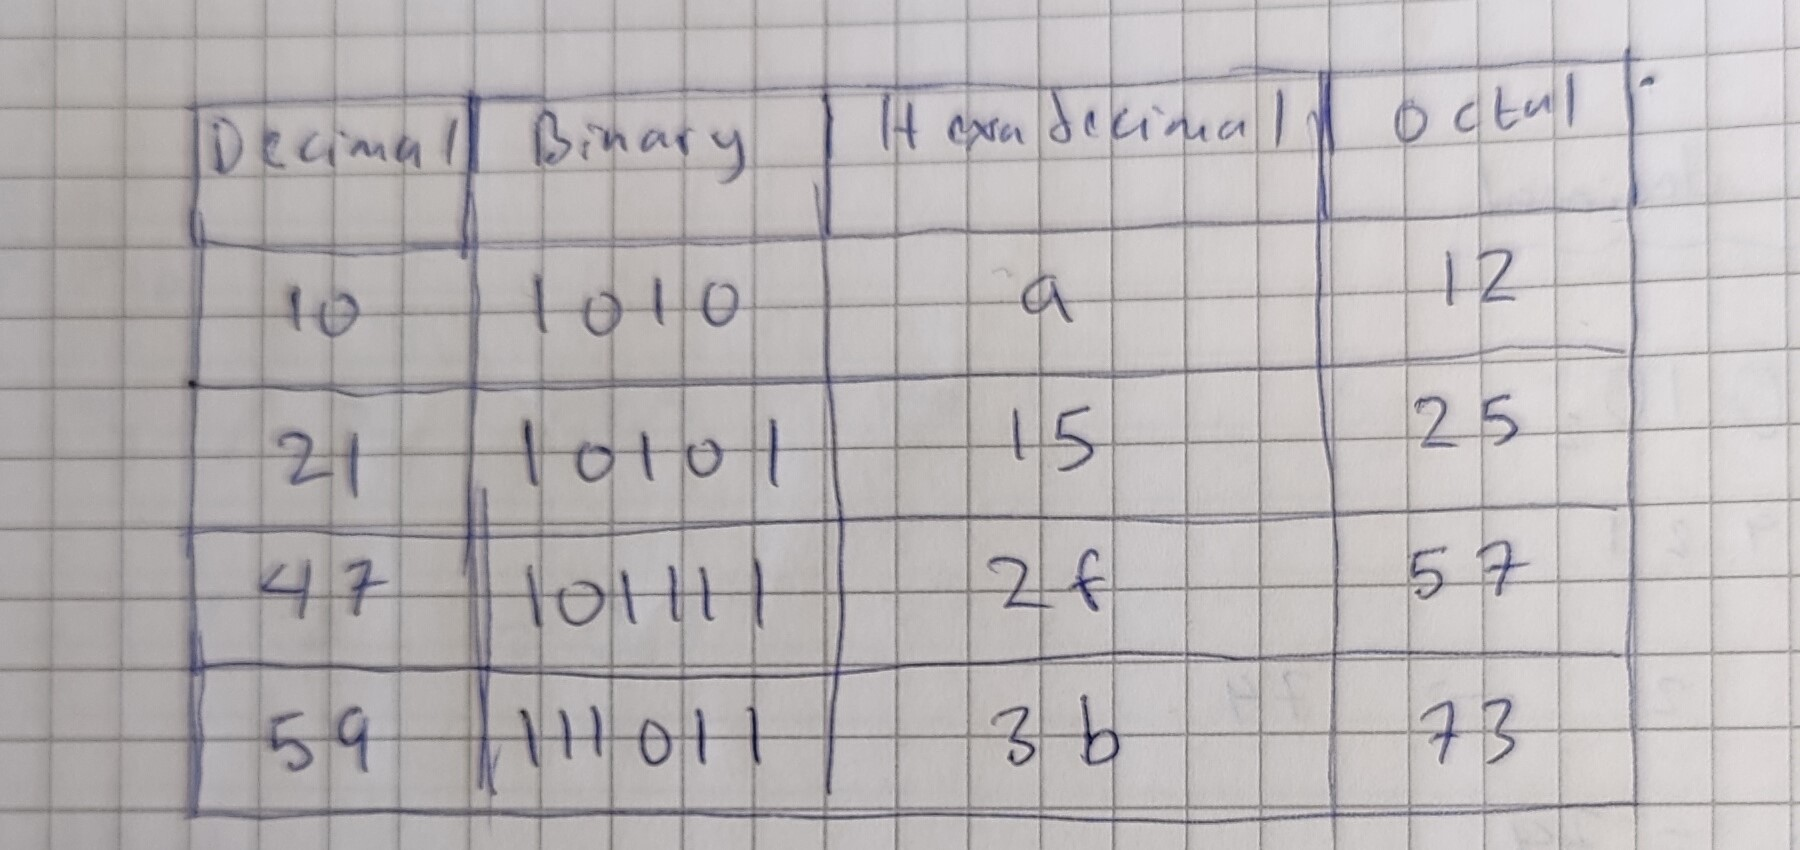
\includegraphics[width=10cm]{2i2 tab.jpg}
\caption*{Tabelen upfyldes på papir}
\end{center}
\end{figure}

\begin{figure}[h!]
\begin{center}
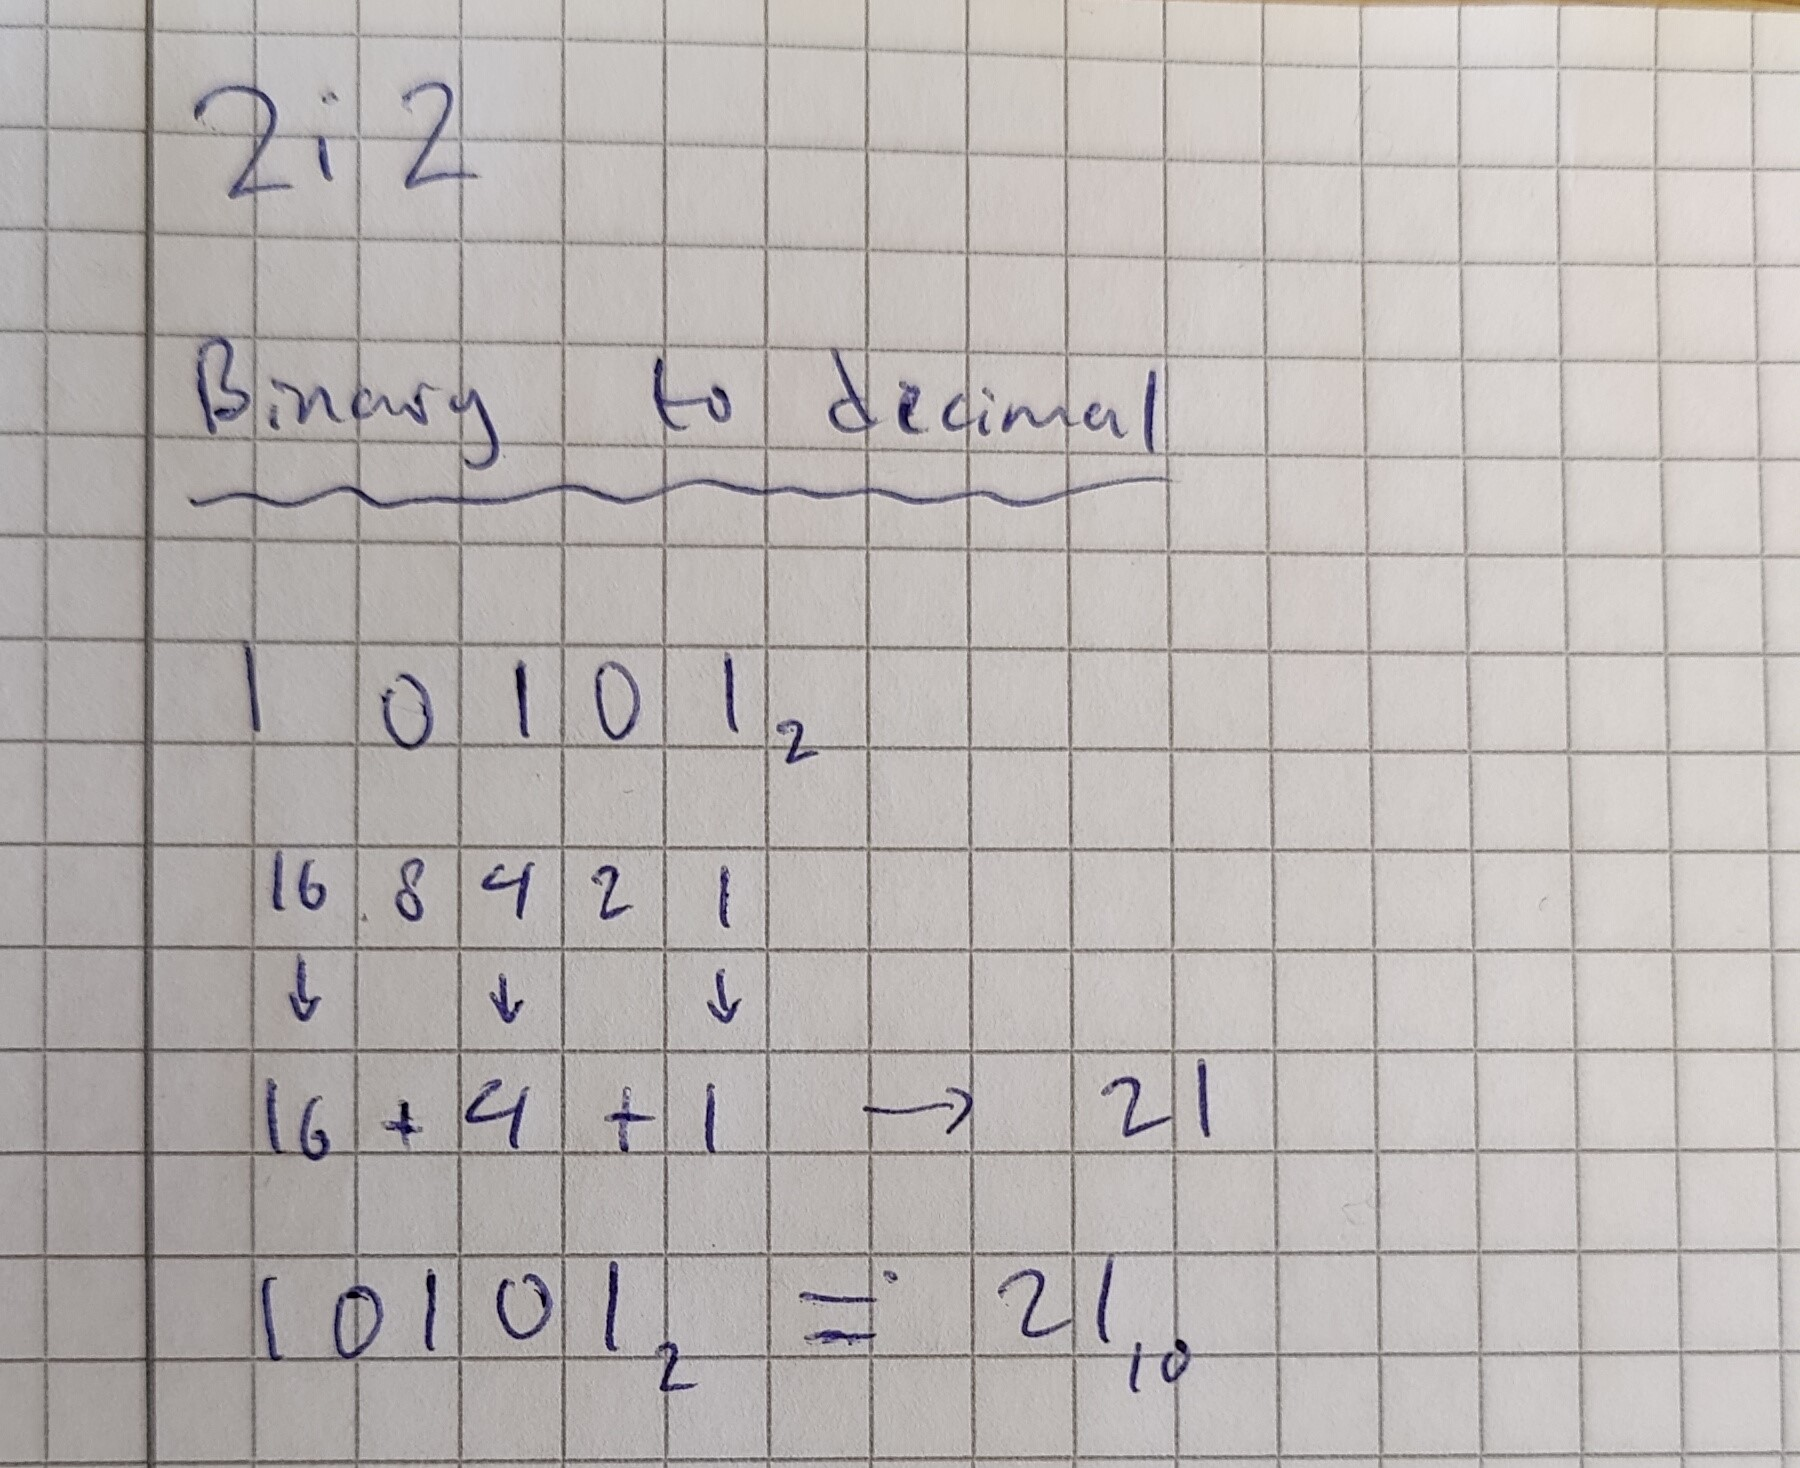
\includegraphics[width=7cm]{2i2 1.jpg}
\caption*{Binært til decimalt}
\end{center}
\end{figure}

\begin{figure}[h!]
\begin{center}
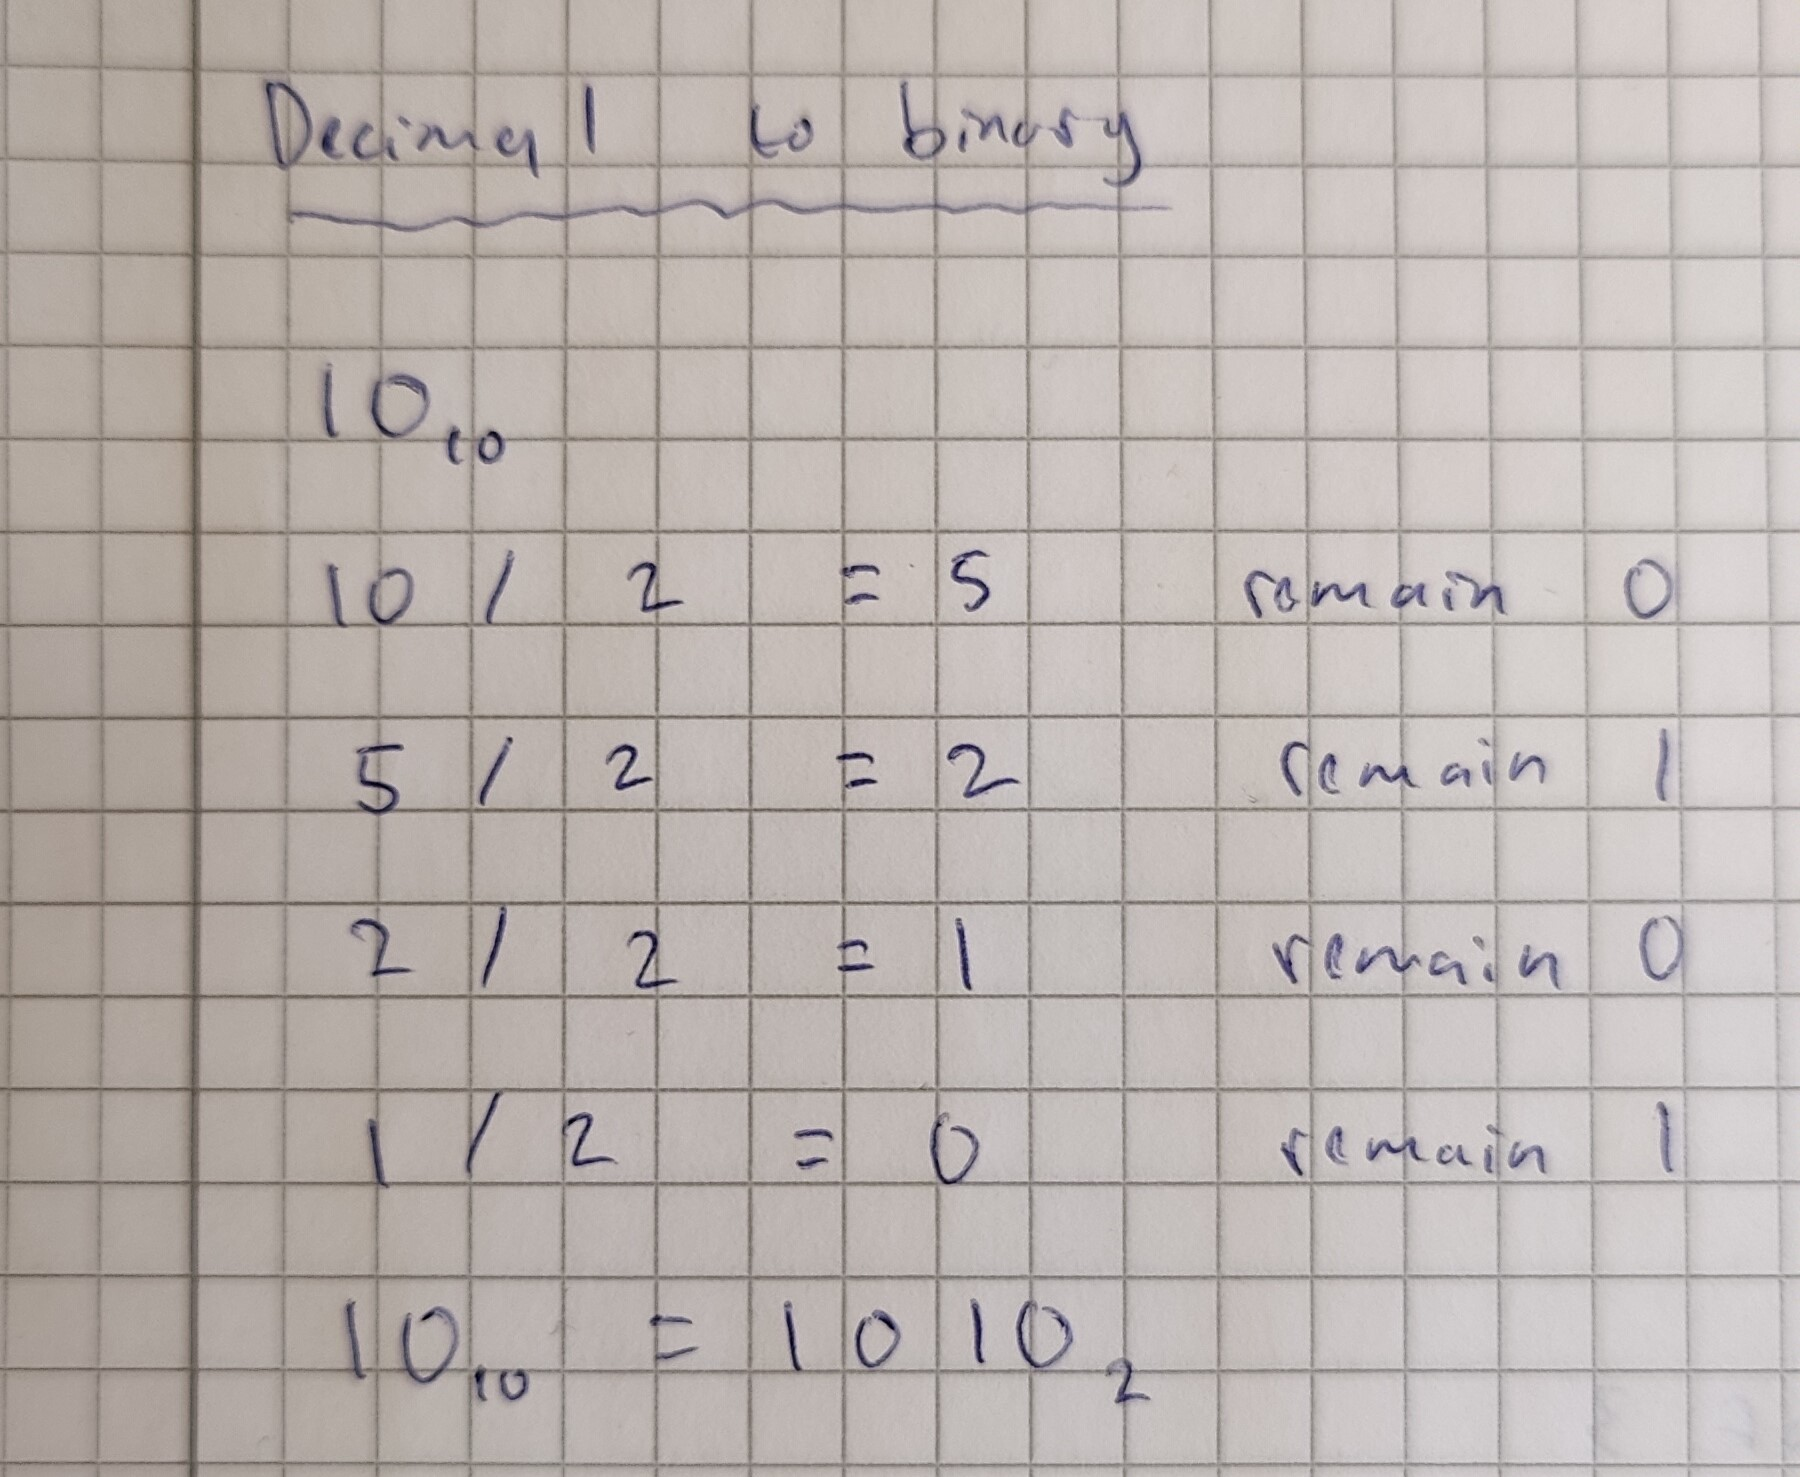
\includegraphics[width=7cm]{2i2 2.jpg}
\caption*{Decimalt til binært}

\end{center}
\end{figure}

\begin{figure}[h!]
\begin{center}
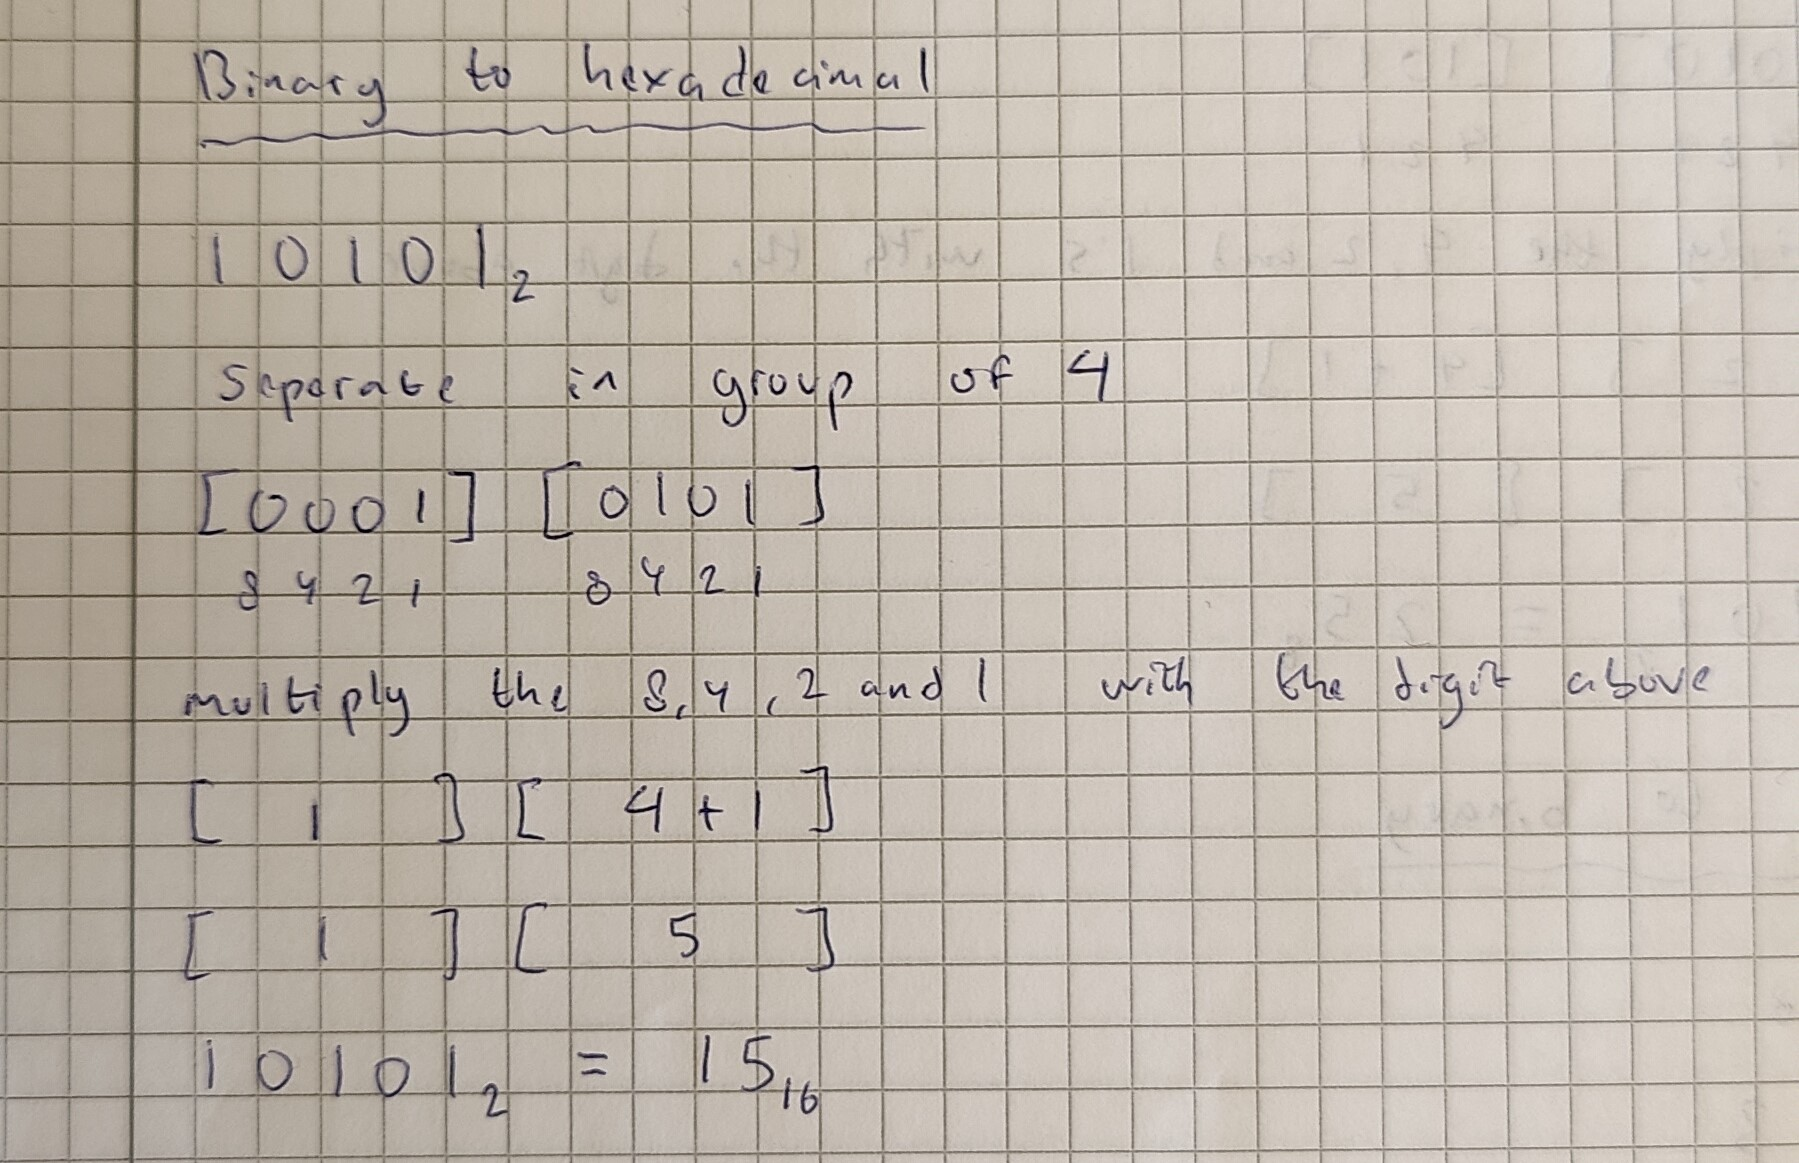
\includegraphics[width=10cm]{2i2 3.jpg}
\caption*{Binært til hexadecimalt}
\end{center}
\end{figure}

\begin{figure}[h!]
\begin{center}
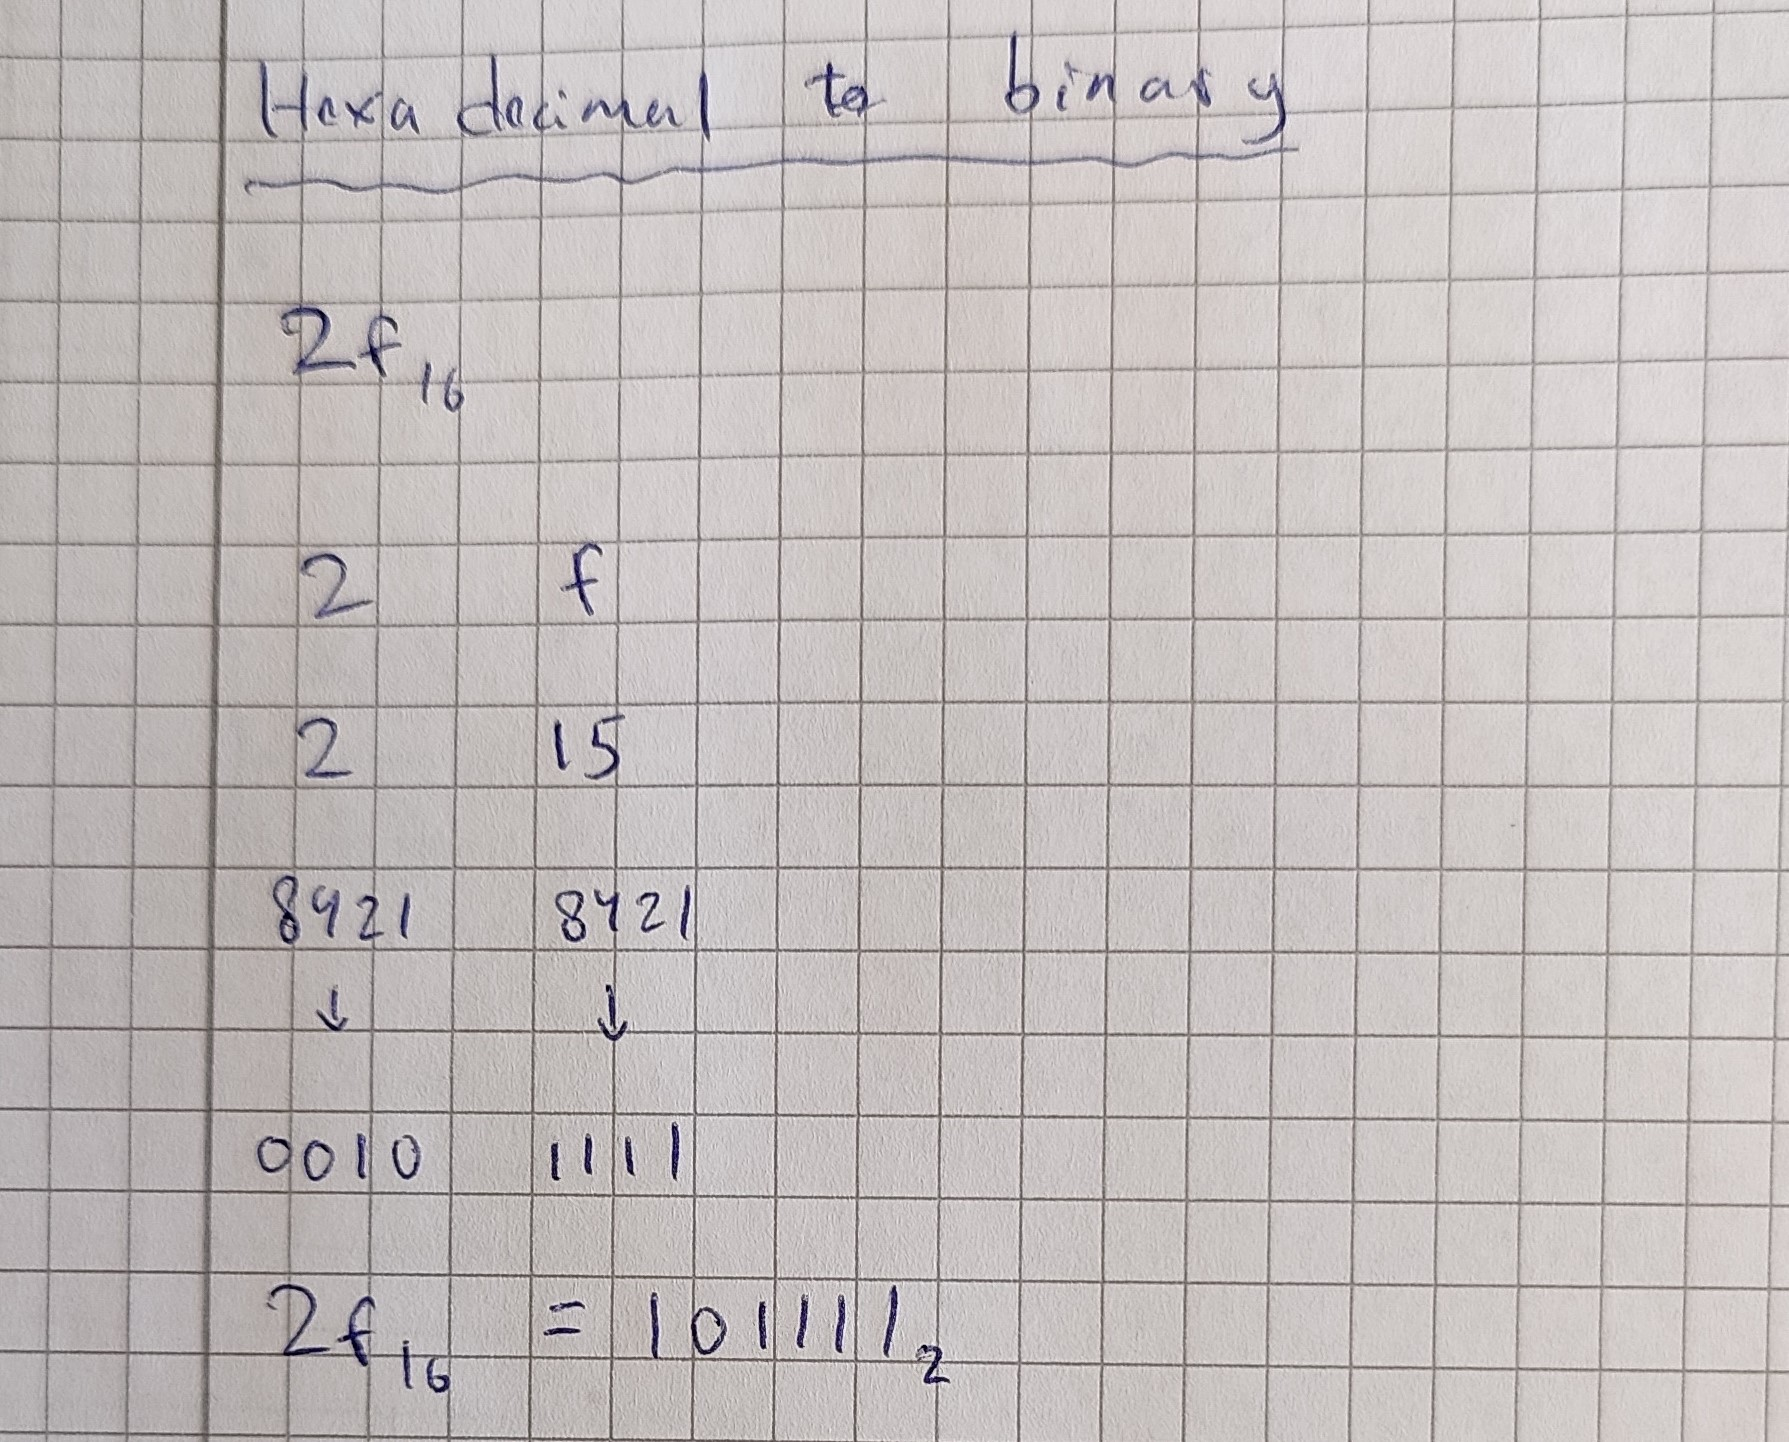
\includegraphics[width=7cm]{2i2 4.jpg}
\caption*{Hexadecimalt til binært}
\end{center}
\end{figure}

\begin{figure}[h!]
\begin{center}
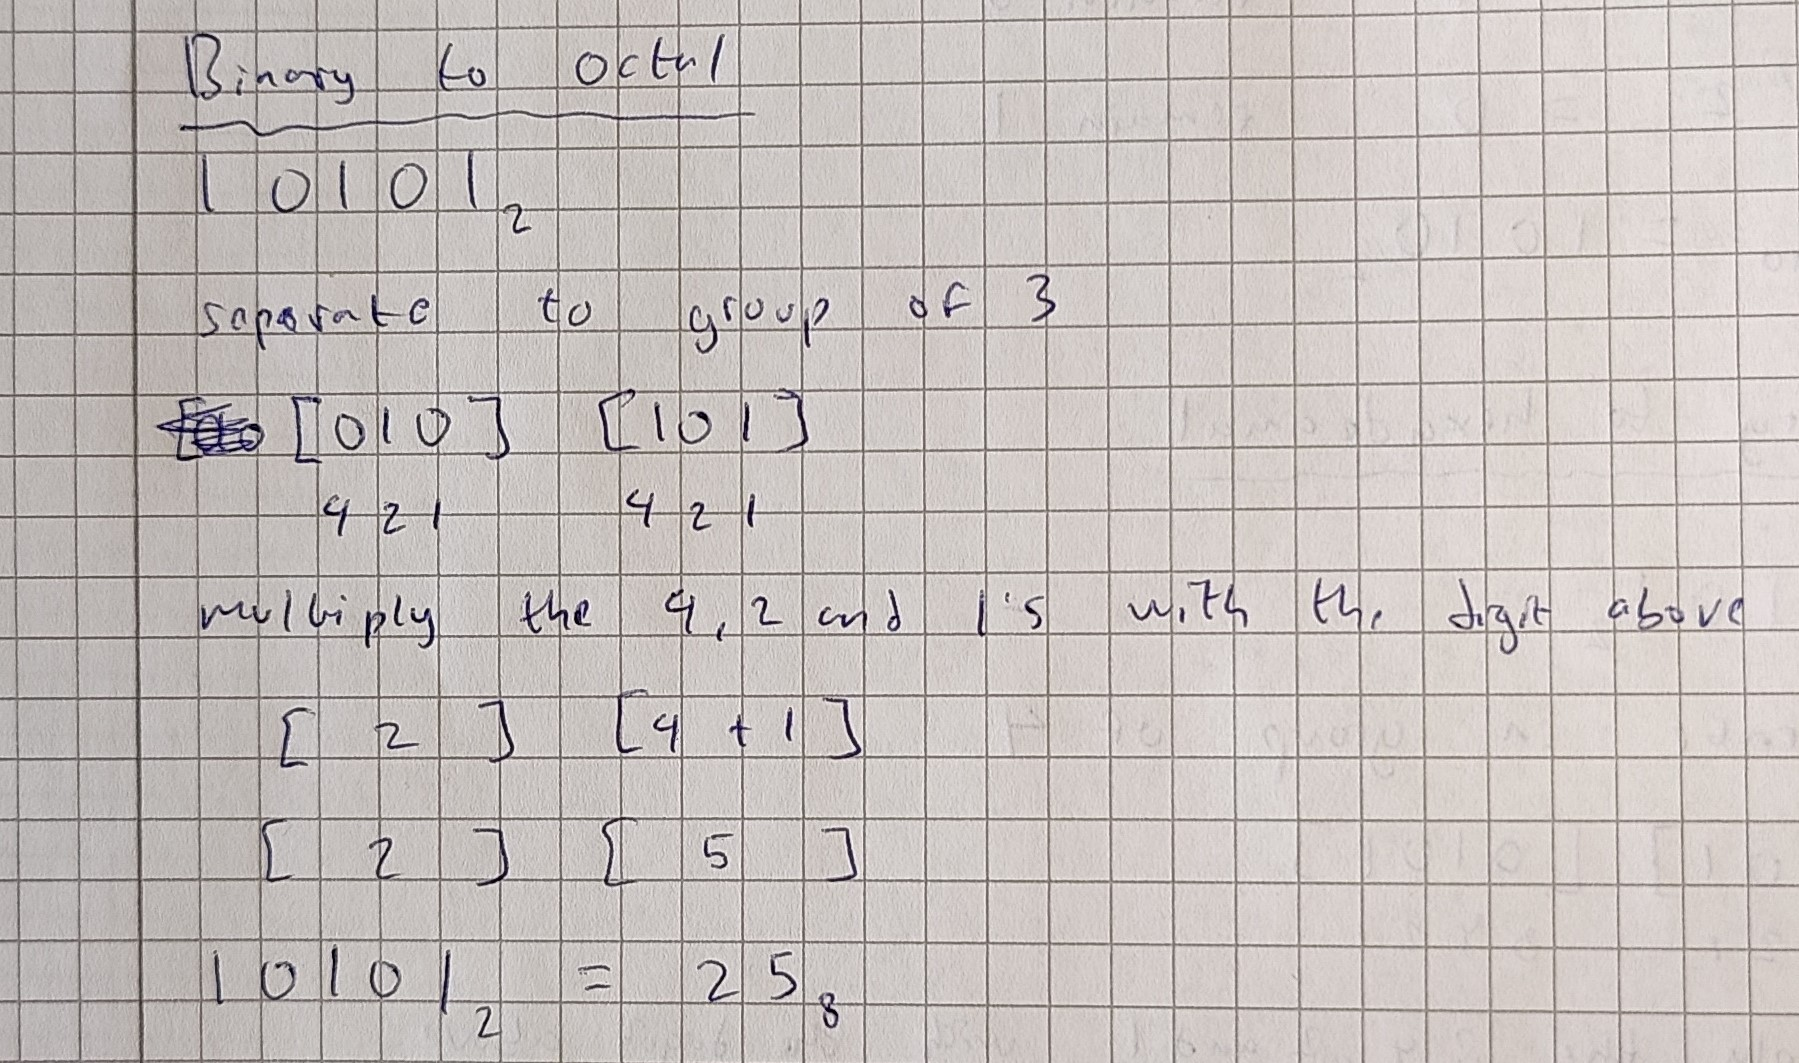
\includegraphics[width=10cm]{2i2 5.jpg}
\caption*{Binært til oktalt}
\end{center}
\end{figure}

\begin{figure}[h!]
\begin{center}
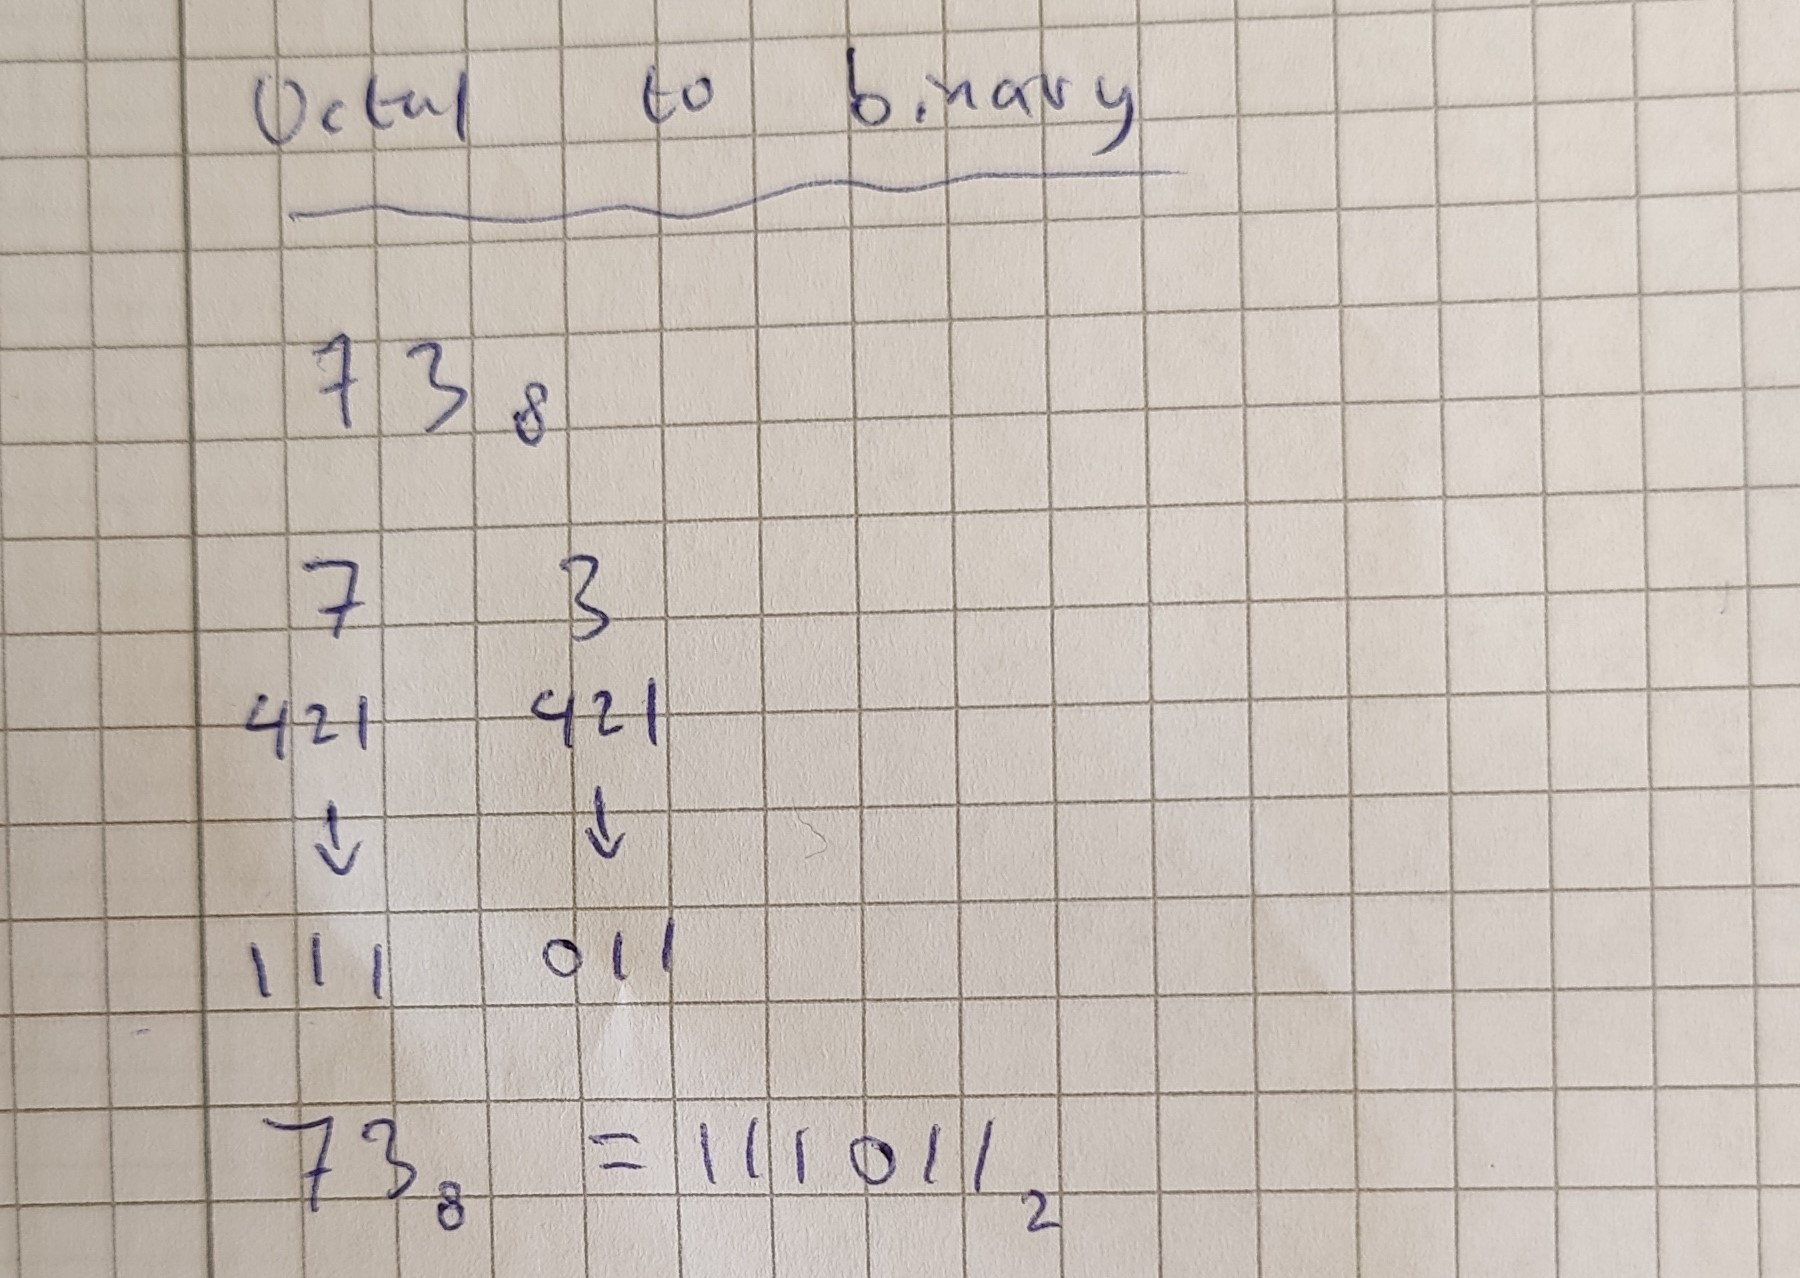
\includegraphics[width=7cm]{2i2 6.jpg}
\caption*{Oktalt til binært}
\end{center}
\end{figure}


\end{document}